\chapter{Trabalhos Correlatos}

Para prover serviços inteligentes para \textit{SmartSpaces} é necessário adquirir informações de contexto, informações sobre a pessoas no ambiente e suas interações. Informações como número de pessoas, identidade, localização, postura, orientação da cabeça, entre outros.

Neste capítulo analisaremos alguns projetos que procuram obter informações de contexto como esta. De modo mais específico, informações sobre a identidade e localização das pessoas em um \textit{SmartSpace}.

\section{Projeto CHIL}

O Projeto CHIL (\textit{Computers in the Human Interaction Loop}) é composto por um time de quinze laboratórios internacionais de pesquisa acadêmica e industrial . Eles colaboram entre si no desenvolvimento de serviços que visam ajudar as pessoas de forma proativa durante suas atividades diárias e, em particular, durante sua interação com as outras pessoas. 

Alguns dos protótipos que foram desenvolvidos no projeto incluem um \textit{workspace} perceptivo e colaborativo, diversos serviços que facilitam a colaboração em reuniões e em salas de palestras, e um sistema perceptivo de assitência a um escrtitório virtual~\cite{chil}.

\subsection{Rastreamento e Lozalização de Pessoas}

A pesquisa sobre rastreamento de pessoas foi focada principalmente no rastreamento de pessoas dentro de \textit{SmartSpaces}. O objetivo desse monitoramento foi determinar, para todos os pontos no tempo, as coordenadas dos ocupantes do \textit{SmartSpaces} na cena em relação a uma \textit{frame} de coordenadas. O que contradiz com a maioria das pesquisas de rastreamento visual, onde somente as coordenadas na imagem  são estimadas~\cite{chil}.

Os sensores usados no \textit{SmartSpace} incluem~\cite{chil}:
	
	\begin{itemize}
		\item um mínimo de quatro câmeras fixas instaladas nos cantos da sala, com campos de visão sobrepostos;
		\item uma câmera com grande ângulo de visão fixa com vista para o quarto inteiro;
		\item três arrays de micrfones em forma de T de 4 canais;
		\item um microfone de Mark III de 64 canais;
	\end{itemize}

Essa grande quantidade de sensores disponíveis pode ser vista como uma vantagem, pois podem oferecer uma grande redundância nas informações capturas que podem ser exploradas pelos algoritmos usados. Porém, isso pode também ser visto como um grande desafio, pois surgem problemas como sincronização dos dados, transferência de processamento distribuído, fusão de espaço-temporal, entre outros.

Do ponto de vista do áudio, é importante mencionar que o Projeto CHIL representa uma das primeiras tentativas de realizar e avaliar sistematicamente rastreamento acústico com uma rede distribuída de microfones~\cite{chil}.
	 
O sistema de rastreamento e localização foi amplamente testado usando os dados dos seminários e reuniões CHIL~\cite{chil}.

Durante o projeto, muito progresso foi feito partindo de sistemas de única modalidade com a inicialização manual ou implícita, usando recursos simples, o que implica várias etapas de processamento manualmente concatenadas offline e acompanhamento de no máximo uma pessoa, para um sistema totalmente automático, com auto-inicialização, em tempo real, usando uma combinação de recursos, fusão dos \textit{streams} de vários sensores de áuido e video e capaz de rastrear alvos múltiplos~\cite{chil}.

Sobre os algoritmos de rastreamento visual, duas abordagens principais foram seguidas pelos vários sistemas de rastreamento desenvolvidos~\cite{chil}:
	
	\begin{enumerate}
		\item uma abordagem baseada em modelos, em que um modelo 3D do objeto rastreado é mantido.
		\item  uma abordagem orientada a dados, onde sistemas de rastreamento 2D operam de forma independente sobre os diferentes ângulos de visão das câmeras e os dados do rastreamento pertencentes a um mesmo alvo são coletados no formato de um rastreamento 3D.
	\end{enumerate}

 Em termos de desempenho, a abordagem baseada em modelos geralmente prevê uma melhor acurácia, mas menos precisão do que a abordagem orientada a dados. O tratamento das oclusões e da associação dos dados dos sistemas de rastreamentos independentes são as desvantagens do modelo orientado a dados. Para diminuir o impacto desses problemas, começaram a detectar e rastrear rostos em vez de corpos inteiros~\cite{chil}.

% Sobre os algoritmos de rastreamento por áudio, três abordagens principais foram seguidas~\cite{chil}:
	
	% \begin{enumerate}
	% 	\item abordagens que dependem do cálculo de um campo de coerência global mais ou menos grosseiro, em que o rastreamento dos picos de correlação é realizada;
	% 	\item abordagens filtro de partículas, que estima a posição da pessoa que fala através de um conjunto de amostras e medições dos sinais acústicos observados dado a cada amostra hipóteses sobre a posição;
	% 	\item abordagens que se alimentam dos atrasos de chegada calculados entre os pares microfone como observações para um rastreador probabilístico.
	% \end{enumerate}

Sobre os algoritmos de rastreamento por áudio, três abordagens principais foram seguidas. Entre elas, a que teve a melhor performance foi um sistema baseado em um \textit{Joint Probabilistic Data Association Filter}, que mantém o controle de uma série de fontes de áudio, incluindo fontes de ruídos, resolvendo associações dos dados e atualizando o conjunto de posições~\cite{chil}.

As abordagens de rastreamento por meio de áudio e vídeo foram combinas em um rastreamento multimodal. Esse rastreamento multimodal é, notavelmente, baseado em filtro de partículas uma vez que permitem uma integração flexível de recursos através dos sensores~\cite{chil}.

No rastreamento multimodal, era esperado que a fusão dos diferentes tipos de dados proveria resultados mais precisos, eliminando, assim, os efeitos de decisões erradas tomadas por algum rastreamento monomodal. Porém, não aconteu o que se esperava. O rastreamento multimodal é altamente dependente das tarefas e dados em mãos, e exige um cuidadoso equilíbrio na disponibilidade e qualidade dos dados~\cite{chil}.

\subsection{Identificação das Pessoas}


A fim de realizar identificação de forma natural e implicita, os sensores distribuídos no ambiente devem monitorar continuamente o espaço, e captura de dados audiovisual das pessoas discretamente quando eles aparecem. Ou seja, o sistema de identificação de pessoas
deve operar em segundo plano, sem necessitar de atenção e cooperação das pessoas. Dependendo da localização de uma pessoa e sua distância dos sensores, os dados recebidos podem variar~\cite{chil}. 

Para reconhecimento facial, o sistema utiliza sequencias de imagens fornecidas pelas várias camêras no \textit{SmartSpace}. A cada $\displaysyle 200ms$ imagens das ``caixas delimitadoras das faces'' e posições dos centros dos olhos são fornecidas, como exemplificado na Figura \ref{chil}. As faces, então, são alinhadas utilizando os centros dos olhos ou utilizando as ``caixas delimitadoras das faces''. Para obter robustez contra alguns erros, o sistema gera algumas imagens alinhadas adicionais modificando rótulos dos centros dos olhos ou os rótulos das ``caixas delimitadoras das faces''~\cite{chil}.

	\begin{figure}[hbt]
		\begin{center}
			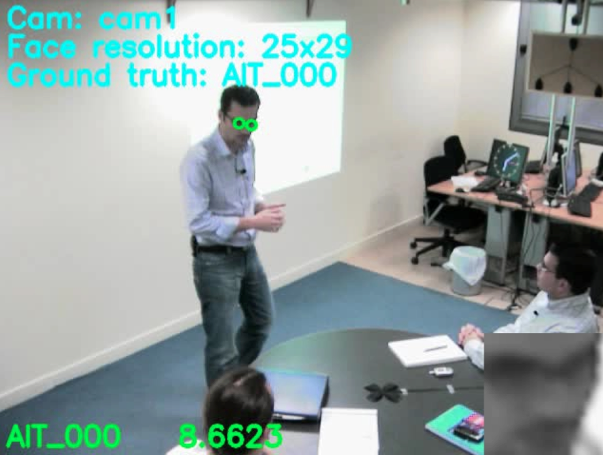
\includegraphics[scale=0.4]{figuras/3.TrabalhosCorrelatos/chil.png}
		\end{center}
		\caption{Exemplo do sistema de indetificação facial do Projeto CHIL. No canto inferior direito, pode-se observar a imagem da face extraída~\cite{chil}.}
		\label{chil}
	\end{figure}

Uma das abordagens utiliza reconhecimento facial baseado na aparência utilizando transformada discreta de cosseno (DCT). Utiliza modelagem de variação intrapessoal de Gauss para avaliar a probabilidade de que a diferença de um rosto de uma galeria de imagens de faces é de fato intrapessoal. O sistema de reconhecimento utiliza um classificador do ``vizinho'' mais próximo ~\cite{chil}.

Nesse projeto foi observado que selecionando somente as imagens frontais de faces, ao invés das amostras disponíveis, é prejudicial para a performance do sistema de reconhecimento~\cite{chil}.

As decisões obtidas do vários pontos de vista das várias camêras são combinados por meio de uma regra de soma ponderada. Os pesos são determinado de acordo com a separação dos dois melhores resultados~\cite{chil}.













































